% 导言区
\documentclass[UTF8]{article}%book ,report ,letter

%\usepackage{algorithmic}
\usepackage{algorithm}
\usepackage[noend,compatible]{algpseudocode}
% Use the  Input / Output
\renewcommand{\algorithmicrequire}{ \textbf{输入:}} %Use Input in the format of Algorithm  
\renewcommand{\algorithmicensure}{ \textbf{输出:}} %UseOutput in the format of Algorithm  
\makeatletter\renewcommand{\ALG@name}{\textbf{算法}} \makeatother

\usepackage{diagbox}
\usepackage{ctexcap}%采用中文标题宏包(标题是中文的)
\usepackage{graphicx}%图片包
\usepackage{color}%彩色文本
\usepackage{amsmath}
\usepackage{enumerate}
\usepackage{caption2}
\usepackage{hyperref} %超链接包
\usepackage{amsmath}
\usepackage{hyperref} %超链接包
%覆盖超链接红框
\usepackage{algorithm2e,setspace}
\hypersetup{
	colorlinks=true,
	linkcolor=black
}
\title{\heiti PatternsInUse}
\author{\kaishu LukeAlanLee}
\date{\today}

% 正文区(文稿区)
\begin{document}
	\maketitle %让头部内容在正文区显示
	\tableofcontents
	\newpage
	\section{第一章}
		\subsection{1.1}
		%列表
			\begin{enumerate}
				\item 
				\begin{itemize}
					\item 
					\begin{description}
						\item[label] description
					\end{description}
				\end{itemize}
			\end{enumerate}
			%图
			\begin{figure}[H]
				\centering
				\noindent\makebox[\textwidth][c] {
					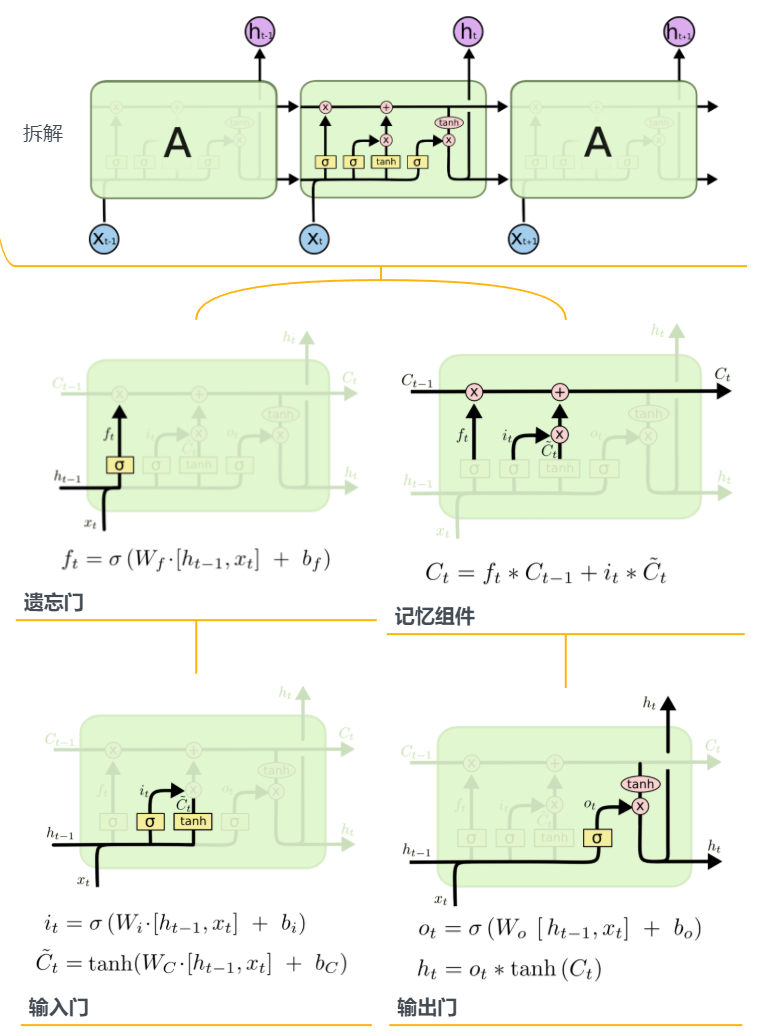
\includegraphics[width=0.5\paperwidth]{figures/LSTMAllInOne.png}}
				\caption{LSTMAllInOne}  %图片的名称
				\label{LSTMAllInOne}   %标签,用作引用
			\end{figure}
		
 		  	\begin{figure}[h]%%图
				\centering  %插入的图片居中表示
				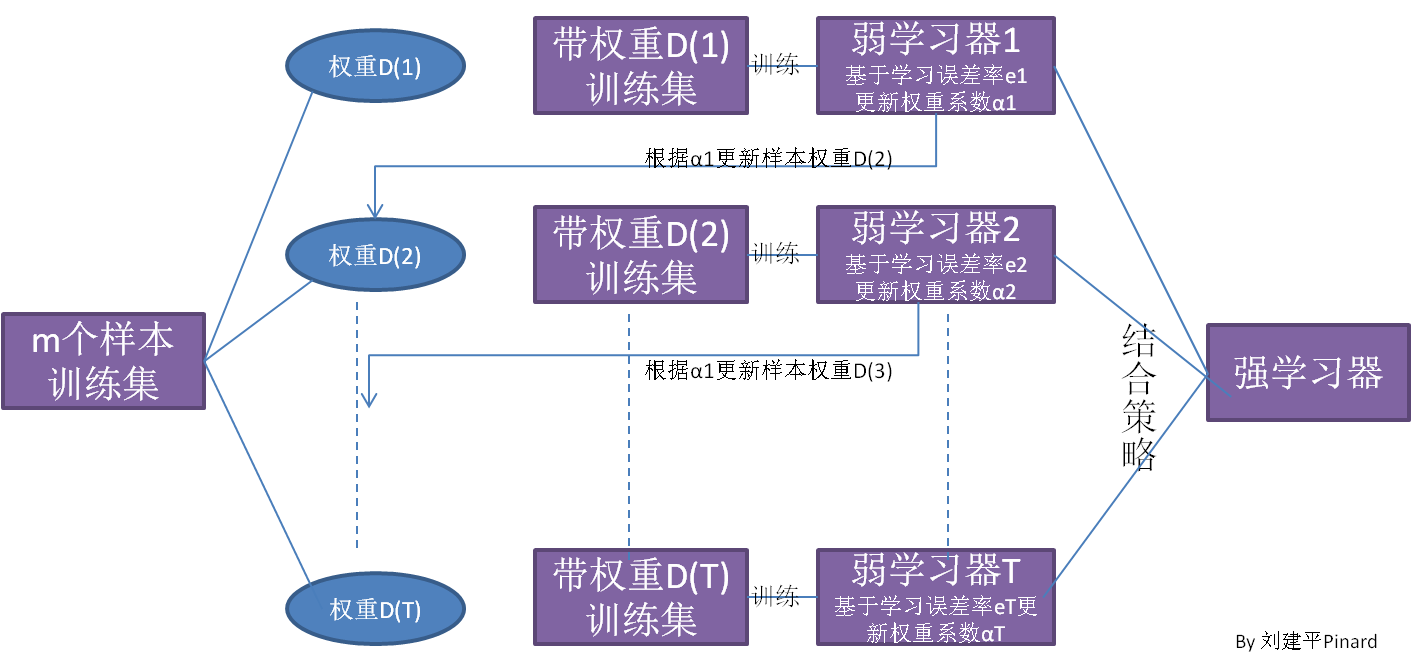
\includegraphics[width=1.0\linewidth]{figures/adaboost}  %插入的图,包括JPG,PNG,PDF,EPS等,放在源文件目录下
				\caption{boosting算法基本思想}  %图片的名称
				\label{boosting}   %标签,用作引用
			\end{figure}
			\clearpage
			%表
			
			%红色
			\color{red}**\color{black}
			
			%带编号公式
			\begin{align}
			\end{align}
			%伪代码
				\begin{algorithm}
				\setstretch{1.35}
				\SetAlgoLined
				\KwData{this text}
				\KwResult{how to write algorithm with \LaTeX2e }
				initialization\;
				\For{not at end of this document}{
					read current\;
					\eIf{understand}{
						go to next section\;
						current section becomes this one\;
					}{
						go back to the beginning of current section\;
					}
				}
				\caption{How to write algorithms}
			\end{algorithm}
		
		\begin{algorithm}[b]
			\caption{子簇合并} %算法的名字
			\label{algMergeSubCluste}
			\begin{algorithmic}[1]
				\REQUIRE 数据集$\mathbf{X}$, 被合并的簇的ID编号onceClusterID, 当前簇的ID编号$Cid$.
				\ENSURE 合并后的子簇。
				\FOR {$ i:=1 $ \textbf{to} $\mathbf{X}$.size()}
				\IF { $\mathbf{X}[i].id$ == onceClusterID }
				\STATE $\mathbf{X}[i].id$ = $Cid$
				\ENDIF
				\ENDFOR
			\end{algorithmic}
		\end{algorithm}
	
			\begin{algorithm}
			\setstretch{1.35}
			\SetAlgoLined
			\KwIn {$I, instance set of current node$}
			\KwIn{$d, feature dimension$}
			$gain \gets 0$
			$G \leftarrow \sum_{i \in I} g_{i}, H \leftarrow \sum_{i \in I} h_{i}$
			\For{$ j in sorted(I,by x_{jk})$}{
				$G_{L} \leftarrow G_{L}+g_{j}, \quad H_{L} \leftarrow H_{L}+h_{j}$
				$G_{R} \leftarrow G-G_{L}, H_{R} \leftarrow H-H_{L}$
				$score\leftarrow \max \left(score, \frac{G_{L}^{2}}{H_{L}+\lambda}+\frac{G_{R}^{2}}{H_{R}+\lambda}-\frac{G^{2}}{H+\lambda}\right)$
			}
			\caption{How to write algorithms}
		\end{algorithm}
	